\section{Introduction and related work}

\begin{figure*}
	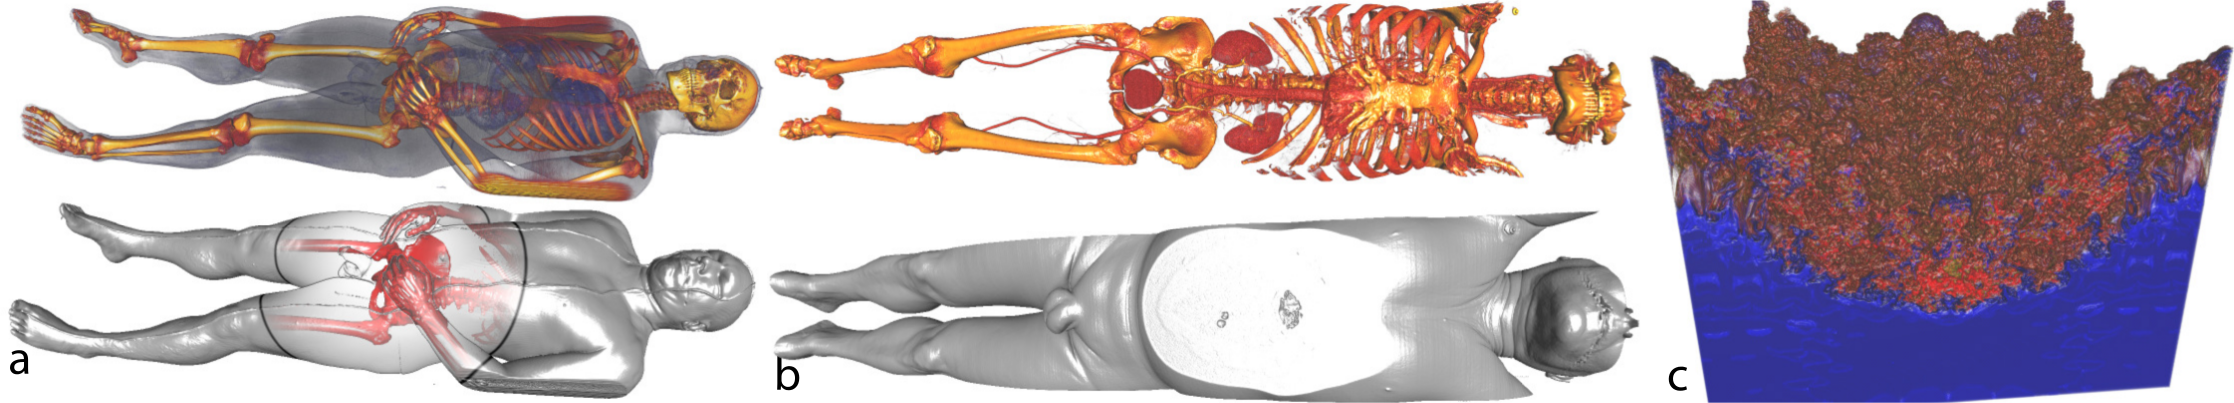
\includegraphics[width=\linewidth]{images/arch/vh-rm}

  \caption{Large data sets rendered with the \textit{Tuvok} framework.
  The Visible Human CT scan (a), the Wholebody data set (b) and a
  Richtmyer-Meshkov instability (c).}
	\label{fig:tvktease}
\end{figure*}

In the past decade texture-based volume rendering on graphics hardware
has positioned itself as a powerful tool for interactive visual
analysis of modestly sized data sets. In earlier years slice-based
approaches~\cite{Cullip:1993:AVRW, Cabral:1994:AVRA} were utilized
due to the limited capabilities of older graphics hardware, with the
drawback of distracting visual artifacts. Later, GPU-based ray casting
became possible on consumer GPUs, producing superior image quality
and allowing for the integration of various acceleration strategies
[KW03]. In addition to improvements in volume traversal methods,
various approaches have been presented to efficiently render data
larger than the video or even the system's main memory.

As data sizes grow, however, an efficient rendering system only solves
part of the visualization problem. Along a different line of research,
novel methods have been proposed to effectively interrogate, search,
highlight and present data with an increasing number of high resolution
features. In the course of this research multi
dimensional-~\cite{Kniss:2005:Multidim}
spatialized-~\cite{Roettger:2005:Spatialized},
size-based-~\cite{Correa:2008:Size-based}, motion
controlled-~\cite{Correa:2005:Motion}, topology-based [WDC ∗ 07],
and style transfer functions [BG07], as well as other focus and
context enhancing techniques [VGH ∗ 05, WZMK05, KSW06] have been
developed. For a complete and detailed survey on volume rendering we
refer the reader to the state of the art report and courses by Engel
et al. [Eng02,EHK ∗ 04] as well as the text book by Hadwiger et
al. [HKRs ∗ 06].

Due to this vast body of research a large variety of dif-
ferent volume rendering systems and prototypes exist both
in academia as well as in industry. Yet researchers and de-
velopers often find themselves implementing the same basic
fundamentals for their new volume rendering application. It
may seem that there are many different good reasons for not
reusing existing, proven code, but one can usually categorize
the decision into one of three cases:

\begin{itemize}

  \item \textbf{System}:
	Often, the integration of new ideas and methods
	into large monolithic rendering systems proves to be a
	bigger issue than re-implementing the entire environment
	from scratch.

	\item \textbf{Software Environment}: The existing code may be imple-
	mented in the wrong environment, such as the program-
	ming environment or graphics APIs. For instance, a Di-
	rectX implementation will not be suitable for a cross plat-
	form project. Further, many research prototypes are tailor-made
	for one system due to the lack of time and need for
	a more general implementation.

	\item \textbf{Licensing}: while largely irrelevant in the academic envi-
	ronment, license issues often prevent developers in com-
	mercial environments from reusing existing code. Even
	code that is released under Open Source conditions may
	come with untenable requirements, such as the GPL’s stip-
	ulation that related yet non-derivative code be released un-
	der the GNU license.

\end{itemize}

Research groups and companies often release their work
and thus a number of systems for volume rendering struc-
tured data exist as free or open source programs. One of the
earliest examples of such an open source volume rendering
system is Stanford’s VolPack software [Com95]. Unfortu-
nately it has not been under development for more than a
decade. A more recent example is the Simian system devel-
oped by Kniss et al. [KKH02]. Released under a very lib-
eral open source license, it has a very polished user inter-
face, and allows the application of multi dimensional trans-
fer functions. Unfortunately it falls short as far as data import
is concerned and development ceased years ago; therefore
no novel render modes are implemented. Other such dis-
continued frameworks and toolkits are the OGLE [Col02]
system, optimized for large data, and OpenQVis [RSEH02],
optimized for fast GPU rendering. A program tailored for
3D Microscopy, Voxx [Ind09], has been released by Indi-
ana University; while it has very promising features, includ-
ing support for 4D data, it is only published in binary form.
While Bruckner and Gröller’s “volumeshop” [BG05] imple-
ments unique GPU accelerated illustrative render options, its
development ceased in 2005 and no current version is avail-
able. Further, it only supported their proprietary volume for-
mat and the current license disallows the use of the code in
commercial environments.

For medical applications the MITK [TXD ∗ 08] toolkit de-
livers many interesting features, including support for large
data sets and data manipulation routines, but it offers only
basic transfer function support and slow performance com-
pared to highly optimized out-of-core GPU volume ren-
dering systems. Solely on the Apple Mac OS X platform,
OsiriX [Ros09] offers unmatched DICOM support in an
open source application, but as the tool is tied closely to Ap-
ple’s Cocoa framework and implemented in Apple-extended
Objective-C, it is nigh-impossible to port to any other plat-
form.

Instead of using a specialized volume rendering applica-
tion, existing visualization toolkits can be utilized to ren-
der volumetric data. The most prominent examples are the
VTK [SML06] and ITK [YAL ∗ 02] systems, which allow
for extremely versatile and flexible rendering and modifi-
cation of many types of data sets. The major drawback is
the lack of support for out-of-core processing, forcing ap-
plication developers to concoct external strategies to handle
large data sets. The ParaView application [AGL05], built on
top of VTK, addresses this issue and extends the support to
large data sets but—like the underlying toolkit—does not
efficiently utilize the capabilities of current graphics cards,
resulting in interactive performance only at very low qual-
ity even for modestly sized data sets. Recently, the VisCG
at the Universität Münster developed the Voreen system
[MSRMH09], a prototyping environment for volume visual-
ization. The interface provided exposes the underlying data
flow network and many visualizations require knowledge as
to how they are technically realized, which we found was not
suitable for a large segment of our user base. Other non com-
mercial visualization toolkits are the OpenDX3 [IBM06]
system which is no longer under active development, and
finally the SCIRun [Ins09] and VisIt [CBB ∗ 05] systems. As
these systems suffered some of the problems of previously
mentioned solutions (e.g. outdated render modes, slow per-
formance, or limited support for large data sets) Tuvok is
currently being integrated into these solutions. Besides these
free \& open source solutions, a number of commercial prod-
ucts exist such as AVS2, Amira, Ensight, syngo, VGStudio
Max, or AltaViewer. As these systems are closed source, ob-
taining detailed information on their operation is difficult;
the possibility of integrating Tuvok into these systems is in-
triguing, but we do not discuss them in detail for this work.

In order to address the aforementioned three issues and to overcome the
limitations of existing systems, we present \textit{Tuvok}, a system
built of cleanly separated components that can
be used together, such as in the \textit{ImageVis3D} application,
or stand-alone. The entire system is implemented in C++ with OpenGL
and DirectX graphics bindings and is designed to be completely
platform independent. When necessary, Tu- vok’s components can be
compiled into a shared library and accessed from another programming
language. Tuvok is also released with a modest open source license that
allows unre- stricted academic and commercial use of the code. Specifi-
cally, \textit{Tuvok} offers the following benefits:

\begin{enumerate}

\item \textbf{Large Data Support}
Given sufficient storage space, the system can theoreti-
cally handle data sets of up to 16 Exabytes in size.
\item \textbf{Modular Design}
While the application ImageVis3D presents itself to the
end-user as a single application, it is composed of a col-
lection of independent Tuvok frameworks.
\item \textbf{Self contained}
While ImageVis3D requires Nokia's Qt [Nok09] library
as an external dependency, \textit{Tuvok} itself does not rely on
external libraries at all.
\item \textbf{Cross platform support}
\textit{Tuvok} as well as \textit{ImageVis3D} support all major platforms,
including various versions of Microsoft Windows, Apple
Mac OS X, and many Linux variants.
\item \textbf{Legacy hardware support}
Tuvok has been extensively tested to work even with the
very limited GPU capabilities of older or less capable
systems.
\item \textbf{Up To Date Rendering algorithms}
Besides its support for 2D and 3D texture based slice
based volume rendering—mostly for older graphics
hardware—\textit{Tuvok} features GPU based ray casting to in-
teractively render images of the highest quality.
\item \textbf{Provenance Support}
\textit{Tuvok} and \textit{ImageVis3D} provide provenance hooks, with
provenance recording and playback realized via VisTrails
[BCS ∗ 05].
\item \textbf{Open Source}
Tuvok and ImageVis3D are released under the very lib-
eral MIT license, which means that practically no usage
restrictions exist—including the use of ImageVis3D or its
components in commercial applications.

\end{enumerate}

The remainder of this chapter is organized as follows. In
Section~\ref{sec:design} we discuss the design of \textit{Tuvok},
focusing on the ways in which the library handles large data. To
demonstrate
the versatility of \textit{Tuvok} and \textit{ImageVis3D}, we describe exten-
sions to the system in section \todo{4}, and projects that have in-
corporated \textit{Tuvok} in section \todo{5}. We conclude the paper with a
summary of the presented system and future research direc-
tions.

\section{Design}
\label{sec:design}

The ImageVis3D system is composed of three major com-
ponents, the Tuvok Volume rendering library, the Tuvok IO
library, and the Qt based UI toolkit. Note that these com-
ponents are designed to work well together but can also be
used separately or replaced by other external libraries (see
Section \todo{5} for examples). In fact, during the compilation pro-
cess of Tuvok the subcomponents are compiled as separate
libraries that are simply linked together. During the design of
these components care has been taken to create flexible and
simple interfaces between the subcomponents. As an exam-
ple of this decoupled design, the communication from the
UI to the rendering and IO systems happens through a single
entity, named the MasterController. This concept makes
it easy to intercept all the communication to and from the
UI (see Section \todo{4.2}) and is also the heart of the scripting in-
terface built into ImageVis3D, which allows programmatic
control over the application.

\subsection{The volume rendering library}

The Tuvok volume rendering library contains the core graph-
ics algorithms to render volumetric data. Currently, a slice
based volume renderer as well as GPU based ray casting
renderer are available in OpenGL and DirectX 10. For pure
software based rendering the system currently relies on the
Mesa library [Pau].

\subsection{Interactivity and quality}

One of the primary design goals of Tuvok is that it should be
able to visualize data sets of incredible size on almost any
commodity system. At present, we have verified the renderer
works with data sizes greater than 2 terabytes [FCS ∗ 10].

This is achieved using a streaming, progressive rendering
system guaranteeing interactive frame rates with adaptive
quality. The generation of full quality imagery is also guar-
anteed on all configurations, with any data set, but may not
happen interactively.

To achieve this goal Tuvok utilizes a multiresolution level
of detail (LoD) data representation. It queries the volume
parameters from the Tuvok IO Library—or an external IO
framework through a documented API if the standard IO is
not used—and uses that information together with the cur-
rent viewing parameters and system performance history to
compute a work order for the current render task. More de-
tails are available in section 3.2.

To achieve goals 4-6 in the list above, renderers contain
a variety of extra code paths for compatibility settings, as a
means to address a number of issues discovered in various
OpenGL drivers. Tuvok contains multiple renderers, based
on ray casting, 3D slicing, and 2D slicing, which span a large
range of quality versus portability across GPUs and drivers.
This has been important to support a breadth of collabora-
tions, as less technical users tend to have integrated graphics
chips which lack support for even 3D textures. Another fea-
ture driven by this requirement is the ability to select the bit
width of the framebuffer object (FBO) used for rendering,
because we found that some drivers would switch to a soft-
ware path when rendering into a 32-bit FBO.

Table 1 gives timings for multiple data sets on different
systems, demonstrating the system’s compatibility and scal-
ability. For these timings the progressive rendering has been
disabled: only the time to render the maximum quality im-
age for the given view was measured. With the progressive
rendering turned on all data sets render at the chosen refresh
rates on all systems. Note that the systems used in the test
cover chipset integrated GPUs as well as also high end PC
configurations. Timings are presented for small data sets as
well as reasonably sized CT scans and simulations. Using
even larger data sets does not significantly impact the per-
formance of the system, as the amount of data accessed is
bounded by the screen resolution.

\begin{table}
	\begin{tabular}{l|c|c|c}
	data set & Air & Pro & Vista \\\hline

	\begin{minipage}{0.4\linewidth}
	\textbf{C60 Molecule}\\128x128x128 8bit = 2 MB\\See	Figure~\ref{fig:modes}
	\end{minipage}
	& 110 / 184 & 80 / 124 & 12 / 14\\\hline

	\begin{minipage}{0.4\linewidth}
	\textbf{VH Male CT}\\512x512x1884 8bit = 471 MB\\See
	Figure~\ref{fig:tvktease}a
	\end{minipage} & 380 / 500 & 526 / 744 & 48 / 76\\\hline

	\begin{minipage}{0.4\linewidth}
	\textbf{Wholebody}\\512x512x3172 16bit = 1586 MB\\See
	Figure~\ref{fig:tvktease}b
	\end{minipage} & 680 / 700 & 587 / 984 & 126 / 301\\\hline

	\begin{minipage}{0.4\linewidth}
	\textbf{RM Instability}\\2048x2048x1920 8bit = 7680 MB\\See
	Figure~\ref{fig:tvktease}c
	\end{minipage} & 5523 / 6112 & 3112 / 3520 & 196 / 321 \\

	\end{tabular}

  \caption{Tuvok timings in \textbf{milliseconds} for various data sets
  and configurations.  ``Air'': MacBook Air, 2GB RAM, onboard GeForce
  9400, ``Pro'': MacBook Pro, 4GB RAM, GeForce 9600, ``Vista'': PC
  running windows Vista, 24 GB RAM, Quadro 5800.  All tests were
  performed in isosurface mode (first value) and in 1D transfer
  function mode (second value), using the ray casting renderer and
  sampling twice per voxel into a 1024x1024 viewport.  The camera was
  zoomed such that the data set covered the entire viewport, and the
  datasets were divided into bricks of size $256^3$.}

\end{table}

\begin{figure*}
	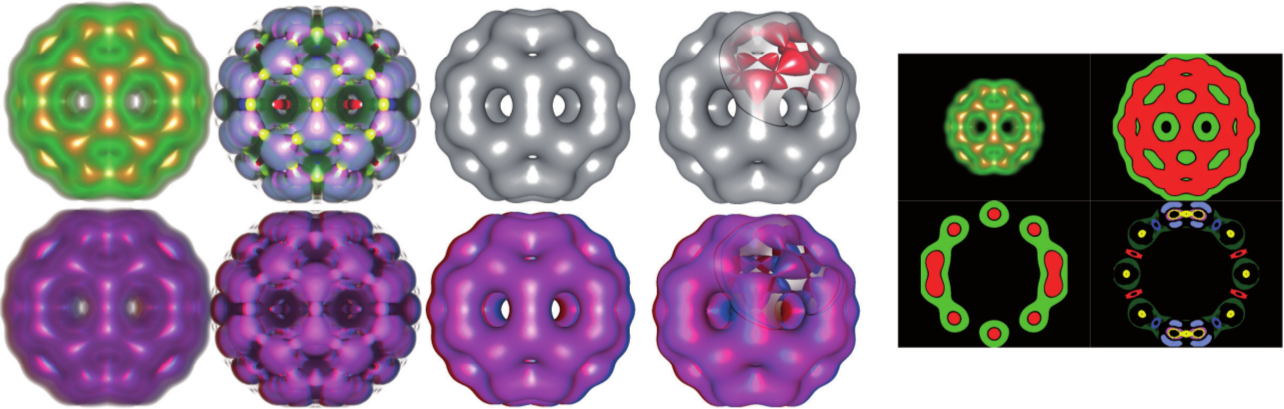
\includegraphics[width=\linewidth]{images/arch/c60modes}

  \caption{Various render modes applied to the C60 dataset.  In the
  top row 1D and 2D transfer functions, isosurface extraction, and
  ClearView are shown.  The bottom row shows the same views in anaglyph
  stereo mode.  On the right is two by two mode featuring a 3D view, a
  MIP view (top right) and two slice views (bottom).}
	\label{fig:modes}

\end{figure*}

\subsection{Large scale data handling}

While Tuvok can take advantage of recent advances in hard-
ware capabilities, it is still true that data are growing and
have been growing faster than modern hardware. Thus, while
the size of data sets that we can interactively render is in-
creasing with each hardware revision, we still find that a
larger percentage of our data sets cannot be rendered interac-
tively. It would be unreasonable to assume this trend would
reverse in the coming years. Therefore, it is critical that in-
teractive visualization systems incorporate progressive ren-
derers.

Tuvok’s progressive renderer is based on overloaded con-
cepts of frames and subframes. In the context of Tuvok, a
frame is a single, complete rendering of the data at native
screen and data resolution. A subframe is an intermediate
state between no rendering and a frame, which includes the
full spatial range of the data and any annotations present in
the visualization. The quality of successive subframes mono-
tonically increases. A sequence of these subframes are ren-
dered before the final frame is displayed, detailing differ-
ent approximations of the complete rendering much more
quickly than a frame can be displayed. We guarantee that
there is always at least one subframe which can be displayed
interactively (within a couple hundred milliseconds). The
system turns to such a subframe when the user is actively
interacting with the data.

To model the concepts of frames and subframes, Tuvok
uses a multiresolution, level of detail representation of data.
For the most part, a subframe corresponds to the data at
a particular level of detail. At the coarsest level of detail,
the data are small enough that they can easily be read from
disk under our real time requirements. However, we found
that older GPUs could not always render such data quickly
enough for our needs. Therefore Tuvok always makes avail-
able up to three additional subframes. These are generated
by lowering the screen resolution of the rendering (and up-
scaling before display to the user), lowering the sampling
rate used by the renderer, or both. Lowering resolution and
sample rate significantly reduces the strain on the fragment
processing stage of the graphics pipeline, allowing Tuvok
to respond quickly even on low end hardware. We do not
know any OpenGL 2.0-capable GPU which Tuvok does not
perform acceptably on, and (through extensions) Tuvok can
render even on some cards that do not report OpenGL 2.0
capabilities.

\subsubsection{Preprocessing}

Most data are not fed to visualization software with mul-
tiple levels of detail included. To accommodate such data,
Tuvok’s IO subsystem implements a preprocess which gen-
erates a multiresolution hierarchy. The data at their native
resolution form the finest level of detail, and we subsample
by two recursively until a level of detail exists which is less
than or equal to a predefined user-configured limit. We also
use this opportunity to perform other operations on the data,
for example by converting the endianness so that, in most
cases, it will need no transformations when used for render-
ing later.

The primary issues we face when loading large data are
32-bit address spaces, limitations on GPU 3D texture sizes,
and managing the IO in an efficient manner. The address
space limits us to only handling two gigabytes of data at any
one time. Limitations on texture sizes prevent us from ‘sim-
ply’ loading the data into a single, large 3D texture. Typical
IO performance on desktop-class and predicted future hard-
ware informs our strategy for how we access and consume
data.

To tackle these issues, the preprocess divides each level of
detail into a set of bricks, with each brick small enough to fit
into the texture memory of any modern GPU. The rendering
core will render each level of detail in an out-of-core fashion:
a brick will be loaded, rendered, and discarded as a single
atomic operation. This allows the renderer to load data of
virtually unlimited size with very little available memory, as
the required amount of memory is independent of the data
set size. To achieve the IO performance we require, the IO
library uses large reads (by default, 16 megabytes) that make
seek times virtually irrelevant.

A simple survey of modern disk drives finds reported seek
times ranging from 3.75 up to 8.9 milliseconds. Sustained
transfer rate capabilities can be as low as 65 MB/s; see
Table~\ref{tbl:disks}.  While there are of course differences across
drives and manufacturers, multi-megabyte reads very quickly overtake
seek times as the predominant factor in disk transfers. At 65 MB/s, it
takes just under a quarter of a second to read 16 megabytes of data,
yet only 8 milliseconds to seek to the position of that block. Even as
one gets into the higher end drives, the story is the same; a Cheetah
15K.5 would take 0.12 seconds to read a 16 megabyte chunk of data, and
only 3.75 milliseconds to seek to the appropriate location on disk.
In relative terms, seek time makes up approximately 3% of the time
required to read the data block. Based on these sim- ple calculations,
it is clear that transfer rates will have to improve drastically before
seek times become a relevant pa- rameter.

\begin{table}
	\begin{center}
	\begin{tabular}{l|cc}
	\textbf{Drive name} & \textbf{Seek time (ms)} &
		\textbf{Sustained transfer rate (MB/s)}\\\hline
	Cheetah 15K.5 SAS & 3.75 & 73 to 125\\
	WD Caviar RE2-GP & 8.9 & 84\\
	Barracuda 7200.8 & 8 & 65\\
	WD 740GD & 5.2 & 72\\
	\end{tabular}
	\end{center}

  \caption{Relevant disk performance characteristics for disks ranging
  from high-end server drives (Cheetah 15K.5) to an aging model
  released 6 years ago (WD 740 GD)}
	\label{tbl:disks}
\end{table}

We have also benchmarked our I/O subsystem using solid
state drives. Table~\ref{tbl:ssd} shows the time spent on I/O when
loading a 648-brick data set via Tuvok. The SSD boasts vastly better
seek times, on the order of microseconds instead of the normal
milliseconds for mechanical drives, and a fac- tor of two to three
improvement in bandwidth. Using large reads, the seek time matters
little in this case, but as shown in Table~\ref{tbl:ssd} Tuvok benefits
from the improved transfer times offered by SSDs.

\begin{table}
	\begin{center}
	\begin{tabular}{|c|c|}\hline
	\textbf{3-disk SATA RAID5} & \textbf{Solid state drive}\\\hline
	64.8704 & 27.6723\\\hline
	\end{tabular}
	\end{center}

  \caption{I/O component (seconds) for rendering a 9 gigabyte timestep
  from a simulation of a Richtmyer-Meshkov instability.}
	\label{tbl:ssd}
\end{table}

\subsubsection{Paging strategy}

Transfer time forms the majority of our pipeline execution
time when using high end GPUs. Therefore, by maintaining
a cache for individual bricks, we can improve the overall
rendering time by obviating the need to pay the transfer cost
for every brick rendered.

A straightforward paging strategy for such a cache would
be Least Recently Used (LRU), however this strategy deliv-
ers poor performance in many situations. Consider a dataset
with 10 bricks, and a brick cache capable of storing 9 bricks.
In the first frame, all ten bricks must be paged. Further, load-
ing the final brick of the first frame will evict the first brick
of that frame. Assuming any reasonable amount of frame-to-
frame coherence, the next frame will again need the same 10
bricks, and they are likely to require a similar depth order-
ing. Thus, in the second frame, the first brick we will need
is the brick we just evicted at the end of the last frame; fur-
ther, the second brick we need will be evicted while loading
the first brick of the second frame, and so on throughout the
entire frame.

We have implemented a custom paging strategy which
takes into account our progressive rendering system. In this
strategy, we evict bricks within a frame using the Most Re-
cently Used (MRU) strategy; we evict bricks between frames
using a LRU strategy. The rationale for the former is that
once we have used a brick in a subframe, it will not be
used in the rendering of that frame again until the progres-
sive renderer starts over, and we may service a large number
of bricks in the interim. However, if we do start the frame
from its earliest subframe again, particularly before finish-
ing the frame, we are likely to need the oldest bricks which
are present in the cache. Between frames, we rely on frame-
to-frame coherence. If a brick was not used in the previous
frame, and is not used in the current frame, it is likely to not
be required in subsequent frames as well; a common exam-
ple is if the user has enabled a clip plane: any viewing trans-
form will not effect which bricks are clipped away by the
plane. Therefore the LRU strategy will tend to evict bricks
which are not visible under the current transfer function, iso-
surface, or viewing parameters.

\subsection{UI and networking library}

To facilitate rapid development of other visualization appli-
cations, all those components built on top of Qt which are
not specific to the application level were separated, allowing
them to be shared and reused in future applications. These
components can be roughly categorized as the UI and net-
working components. The independent networking compo-
nents include the bug reporting, update checking, and data
set sharing subsystems, while the UI components include
the base classes that define the look and feel of ImageVis3D,
such as dialogs, tool widgets, user interaction, and persis-
tence.

\section{Extensions to \textit{Tuvok} and \textit{ImageVis3D}}

In this section we will present a couple of examples to
demonstrate how simple it is to add new features or extend
existing functionality. We present examples from research
projects implementing a prototypic environment to experi-
ment with new methods (see Section~\todo{\ref{fixme}}) as well as new
features to ImageVis3D to use it for other research.

Due to the modular design, the scripting interface, and
the MasterController concept, integration with external soft-
ware is simple. As the UI and ‘execution layer’ communicate
strictly through a single class, the MasterController, any
type of external communication channel can simply attach
itself to this class and track changes. Control of the library
can also happen through the MasterController via script
commands that allow programmatic modification of all of
Tuvok’s features.

\subsection{Extensions to the rendering subsystem}

ImageVis3D has been extended to provide domain specific
visualization capabilities. In some domains, it is necessary
to visualize multiple data sets simultaneously. A student has
modified ImageVis3D to render multiple data sets that live in
overlapping space, and added domain-specific widgets for
ease of use in a particular scientific domain. One such ex-
ample is a dialog to automatically create transfer functions,
based on external knowledge of characteristic data distribu-
tions within data sets common to that field. A second exam-
ple is repurposing the 2D transfer function editor to utilize
different metadata along each axis.

\subsection{Extensions to \textit{Tuvok}'s controller}

For provenance tracking, we have integrated VisTrails, a pro-
duction provenance framework with well-developed APIs
for integration with external systems. The integration of
VisTrail’s provenance tracking features required a two way
communication from and to Tuvok. Interactions made by
the user need to be communicated to VisTrails to track the
provenance, but also VisTrails needs to be able to control Tu-
vok to perform undo/redo operations. Thus, this example is
prototypic for any type of recording or remote control of Tu-
vok, such as cluster extensions or connections to novel input
devices.

\section{Use cases of \textit{Tuvok}}

\begin{figure*}
	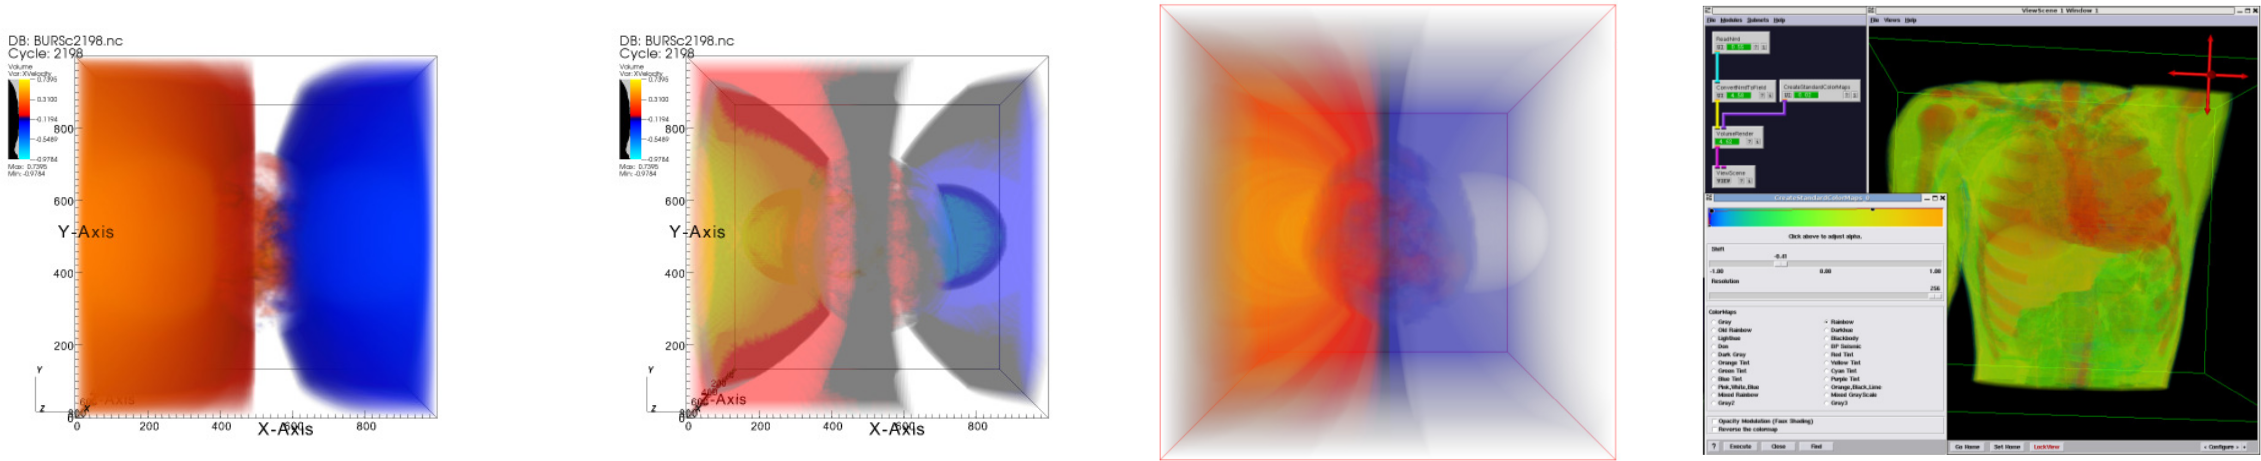
\includegraphics[width=\linewidth]{images/arch/integration}

  \caption{3D texture, SLIVR, and \textit{Tuvok} volume renderers in
  VisIt (left); \textit{Tuvok} rendering a torso in SCIRun (right).}
	\label{fig:integration}
\end{figure*}

In the following we present examples where Tuvok---or only some of it
components---have been integrated into rendering environments other
than
\textit{ImageVis3D}. Figures~\ref{fig:integration}
and~\ref{fig:altaviewer} demonstrate the integrations presented here.

\subsection{SCIRun}

SCIRun is a problem solving environment for modeling,
simulation, and visualization of scientific data. It is an ex-
ample of what we refer to as a legacy application, in that it
was developed without the ideas implemented by Tuvok in
mind. In particular, this means that the system must work
with in-core, “unbricked” data sets of a single resolution.

To support such an environment, Tuvok has a simplified
API for existing systems which do not include level of detail
or bricking concepts. The information flows one way from
the controlling application to Tuvok, and includes a refer-
ence counted smart pointer to the data, as well as metadata
and rendering parameters. For small changes in rendering
parameters, data shared from previous frames is retained and
simply re-rendered. When changing or passing a new data
set to Tuvok, the old data set is removed and replaced by
a new reference counted smart pointer. This scheme allows
us to avoid data copying between the host application and
rendering library. In these kinds of systems, Tuvok does not
have access to a multiresolution form of the data, and thus
cannot guarantee interactive performance.

\subsection{VisIt}

VisIt is a data visualization and analysis application which is
well-suited to large scale data processing on leadership com-
puting platforms. We have integrated the underlying render-
ing core as an option alongside VisIt’s existing volume ren-
derers. Since VisIt already supported domain-based data set
decomposition, it can easily take advantage of an additional
Tuvok feature: bricking. This allows VisIt to volume render
data of arbitrary size on the GPU, whereas it was previously
limited to resampling the data or utilizing software render-
ing.

Though data do not come directly from a data file in this
and other integration work, the abstraction provided by Tu-
vok’s IO layer allows the rendering core to remain ignorant
about the source of the data. The metadata which must be
supplied to Tuvok scales with the complexity of the applica-
tion: in the unbricked, SCIRun case, Tuvok can be told only
the brick size (assuming the brick lies centered on the ori-
gin); with decomposed data, Tuvok must be informed of the
world space location of the bricks; for progressive rendering
applications, such as ImageVis3D, the LoD that a brick be-
longs to must also be given. Should an application choose, it
can also supply additional metadata to allow advanced ren-
dering optimizations.

An issue that arose specifically in the VisIt integration
was state management in large, established software sys-
tems. The OpenGL API is a global state machine, and VisIt
has many sub-libraries which can and will change the global
state in ways we cannot predict. Tuvok therefore makes very
few assumptions about OpenGL state. During the ‘setup’
stage, Tuvok takes state information – camera and viewing
reference points, data, etc. – and simply stores it locally.
A single method then uses all that information to configure
OpenGL state once before moving on to per-brick render-
ing. For efficiency reasons, the system leaves the OpenGL
state “as-is” when finished rendering, much like other VisIt
subsystems and libraries do. Until OpenGL establishes an
object model, we have found this to be the best method for
managing OpenGL state.

\subsection{AltaViewer}

\begin{figure}
	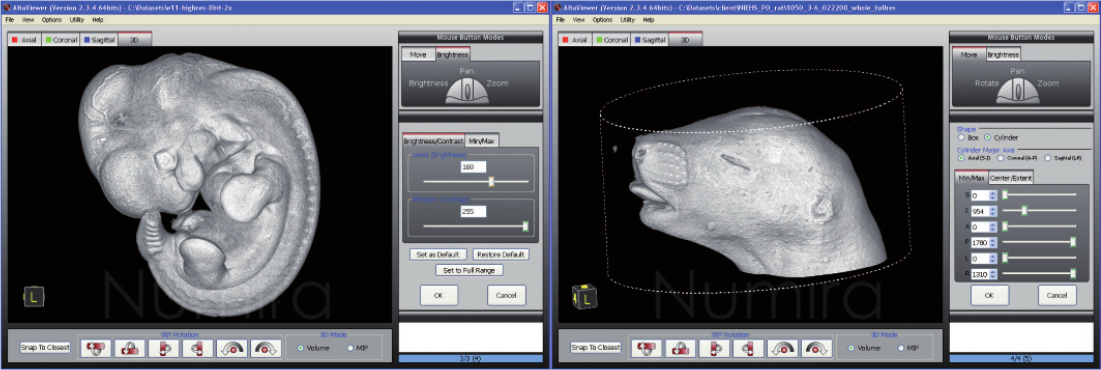
\includegraphics[width=\linewidth]{images/arch/altaviewer}

	\caption{The left image shows an E11 mouse embryo
	(2.4GB) while the right image depicts a P0 newborn rat
	(7.6GB). Both specimens were stained using Numira’s cus-
	tom protocol and scanned using microCT. Images cour-
	tesy of Numira Biosciences. Copyright c 2009 Numira Bio-
	sciences. All rights reserved. AltaViewer Software available
	at \url{http://www.numirabio.com/}}
	\label{fig:altaviewer}
\end{figure}

Finally, we demonstrate the usability of Tuvok’s components
in a commercial environment. Numira Biosciences is a spe-
cialty contract research organization (CRO) which focuses
on high-resolution imaging and analysis of small animal
specimens, provides researchers with quantifiable, visible
evidence of disease progression, as well as drug efficacy and
drug side effects in their animal models. For the next gen-
eration of their visualization suite “AltaViewer” (see
Figure~\ref{fig:altaviewer}) they have chosen to replace their
proprietary IO library in part by Tuvok’s IO components to achieve
significantly better performance.

\section{Conclusion and future work}

In this paper we have presented the Tuvok framework as well
as ImageVis3D, an application built with Tuvok . We gave in-
sight into large data support in a production volume renderer.
We also gave a couple of examples of research projects and
commercial use of components of Tuvok.
We are currently working on three major extensions to
Tuvok. First, the support of time dependent data sets, in par-
ticular we are working to extend the progressive rendering
concept to this data as well. Secondly, we are extending Tu-
vok to render multiple data sets in overlapping 3D space;
due to the out-of-core nature of the system an efficient im-
plementation of this feature is non-trivial. Finally, we also
plan to add purely software based as well as OpenCL based
ray casters to allow for fast rendering of ultra large data sets
on headless clusters with and without GPUs.

\section{Acknowledgements}
This research was made possible in part by the Cluster
of Excellence “Multimodal Computing and Interaction” at
the Saarland University, by the NIH/NCRR Center for In-
tegrative Biomedical Computing, P41-RR12553-10 and by
Award Number R01EB007688 from the National Institute
Of Biomedical Imaging And Bioengineering, and by the Of-
fice of Advanced Scientific Computing Research, Office of
Science, of the U.S. Department of Energy under Contract
No. DE-AC02-05CH11231 through the Scientific Discov-
ery through Advanced Computing (SciDAC) program’s Vi-
sualization and Analytics Center for Enabling Technologies
(VACET). The work presented in this paper has been co-
financed by the Intel Visual Computing Institute. The con-
tent is under sole responsibility of the authors. We thank
John Blondin for some of the data pictured in Figure 4. Fur-
thermore we thank Numira Bioscience for the AltaViewer
screen shots, the visible human project for the visible hu-
man scan and Siemens Corporate Research for the Whole-
body data set.
